\documentclass[8pt]{beamer}
%\documentclass[handout]{beamer}
\title{\LARGE{\textbf{allWomen Tech Assessment}}}

\author{\textbf{Berta Grimau}}
%\institute{Institute of Information Theory and Automation\\ Czech Academy of Sciences}

\date{}

\usepackage[T1]{fontenc}
\usepackage{mathabx}
\usepackage{amsmath}
\usepackage{amsfonts}
\usepackage{amssymb}
\usepackage{amsthm}
\usepackage{ mathrsfs }
\usepackage{hyperref}
\usepackage{mathtools}
\usepackage{lingmacros}
\usepackage{stmaryrd}
\usepackage{ wasysym }

\input{dvipsnam.def}

\setbeamercolor{postit}{fg=Black, bg=Black!10!}

\usepackage[symbol]{footmisc}
\renewcommand{\thefootnote}{\fnsymbol{footnote}}


%\usefonttheme{serif}
%\usepackage{charter}
%\usefonttheme{professionalfonts}

%\usepackage{sansmathfonts}
%\usepackage[T1]{fontenc}
%\renewcommand*\familydefault{\sfdefault}
%\usecolortheme{seagull}
%\setbeamertemplate{footline}[frame number]

\usecolortheme{seagull}
\usepackage{cmbright}
\usepackage[OT1]{fontenc}

\setbeamertemplate{blocks}[rounded]
\setbeamercolor{title}{fg=White}
\setbeamerfont{frametitle}{series=\bfseries}
\setbeamercolor{frametitle}{fg=Periwinkle}
\setbeamerfont{block title}{size=\normalsize,series=\bfseries}

\setbeamertemplate{itemize items}[default]

\setbeamertemplate{sections/subsections in toc}[square]

\setbeamercolor{itemize item}{fg=Tan}  
\setbeamertemplate{itemize item}[triangle] 
\setbeamercolor{itemize subitem}{fg=Tan}  
\setbeamertemplate{itemize subitem}[triangle] 
\setbeamercolor{title}{fg=White}
\setbeamercolor{author}{fg=White}
\setbeamercolor{institute}{fg=White}




\usepackage{natbib}
\begin{document}

{
\usebackgroundtemplate{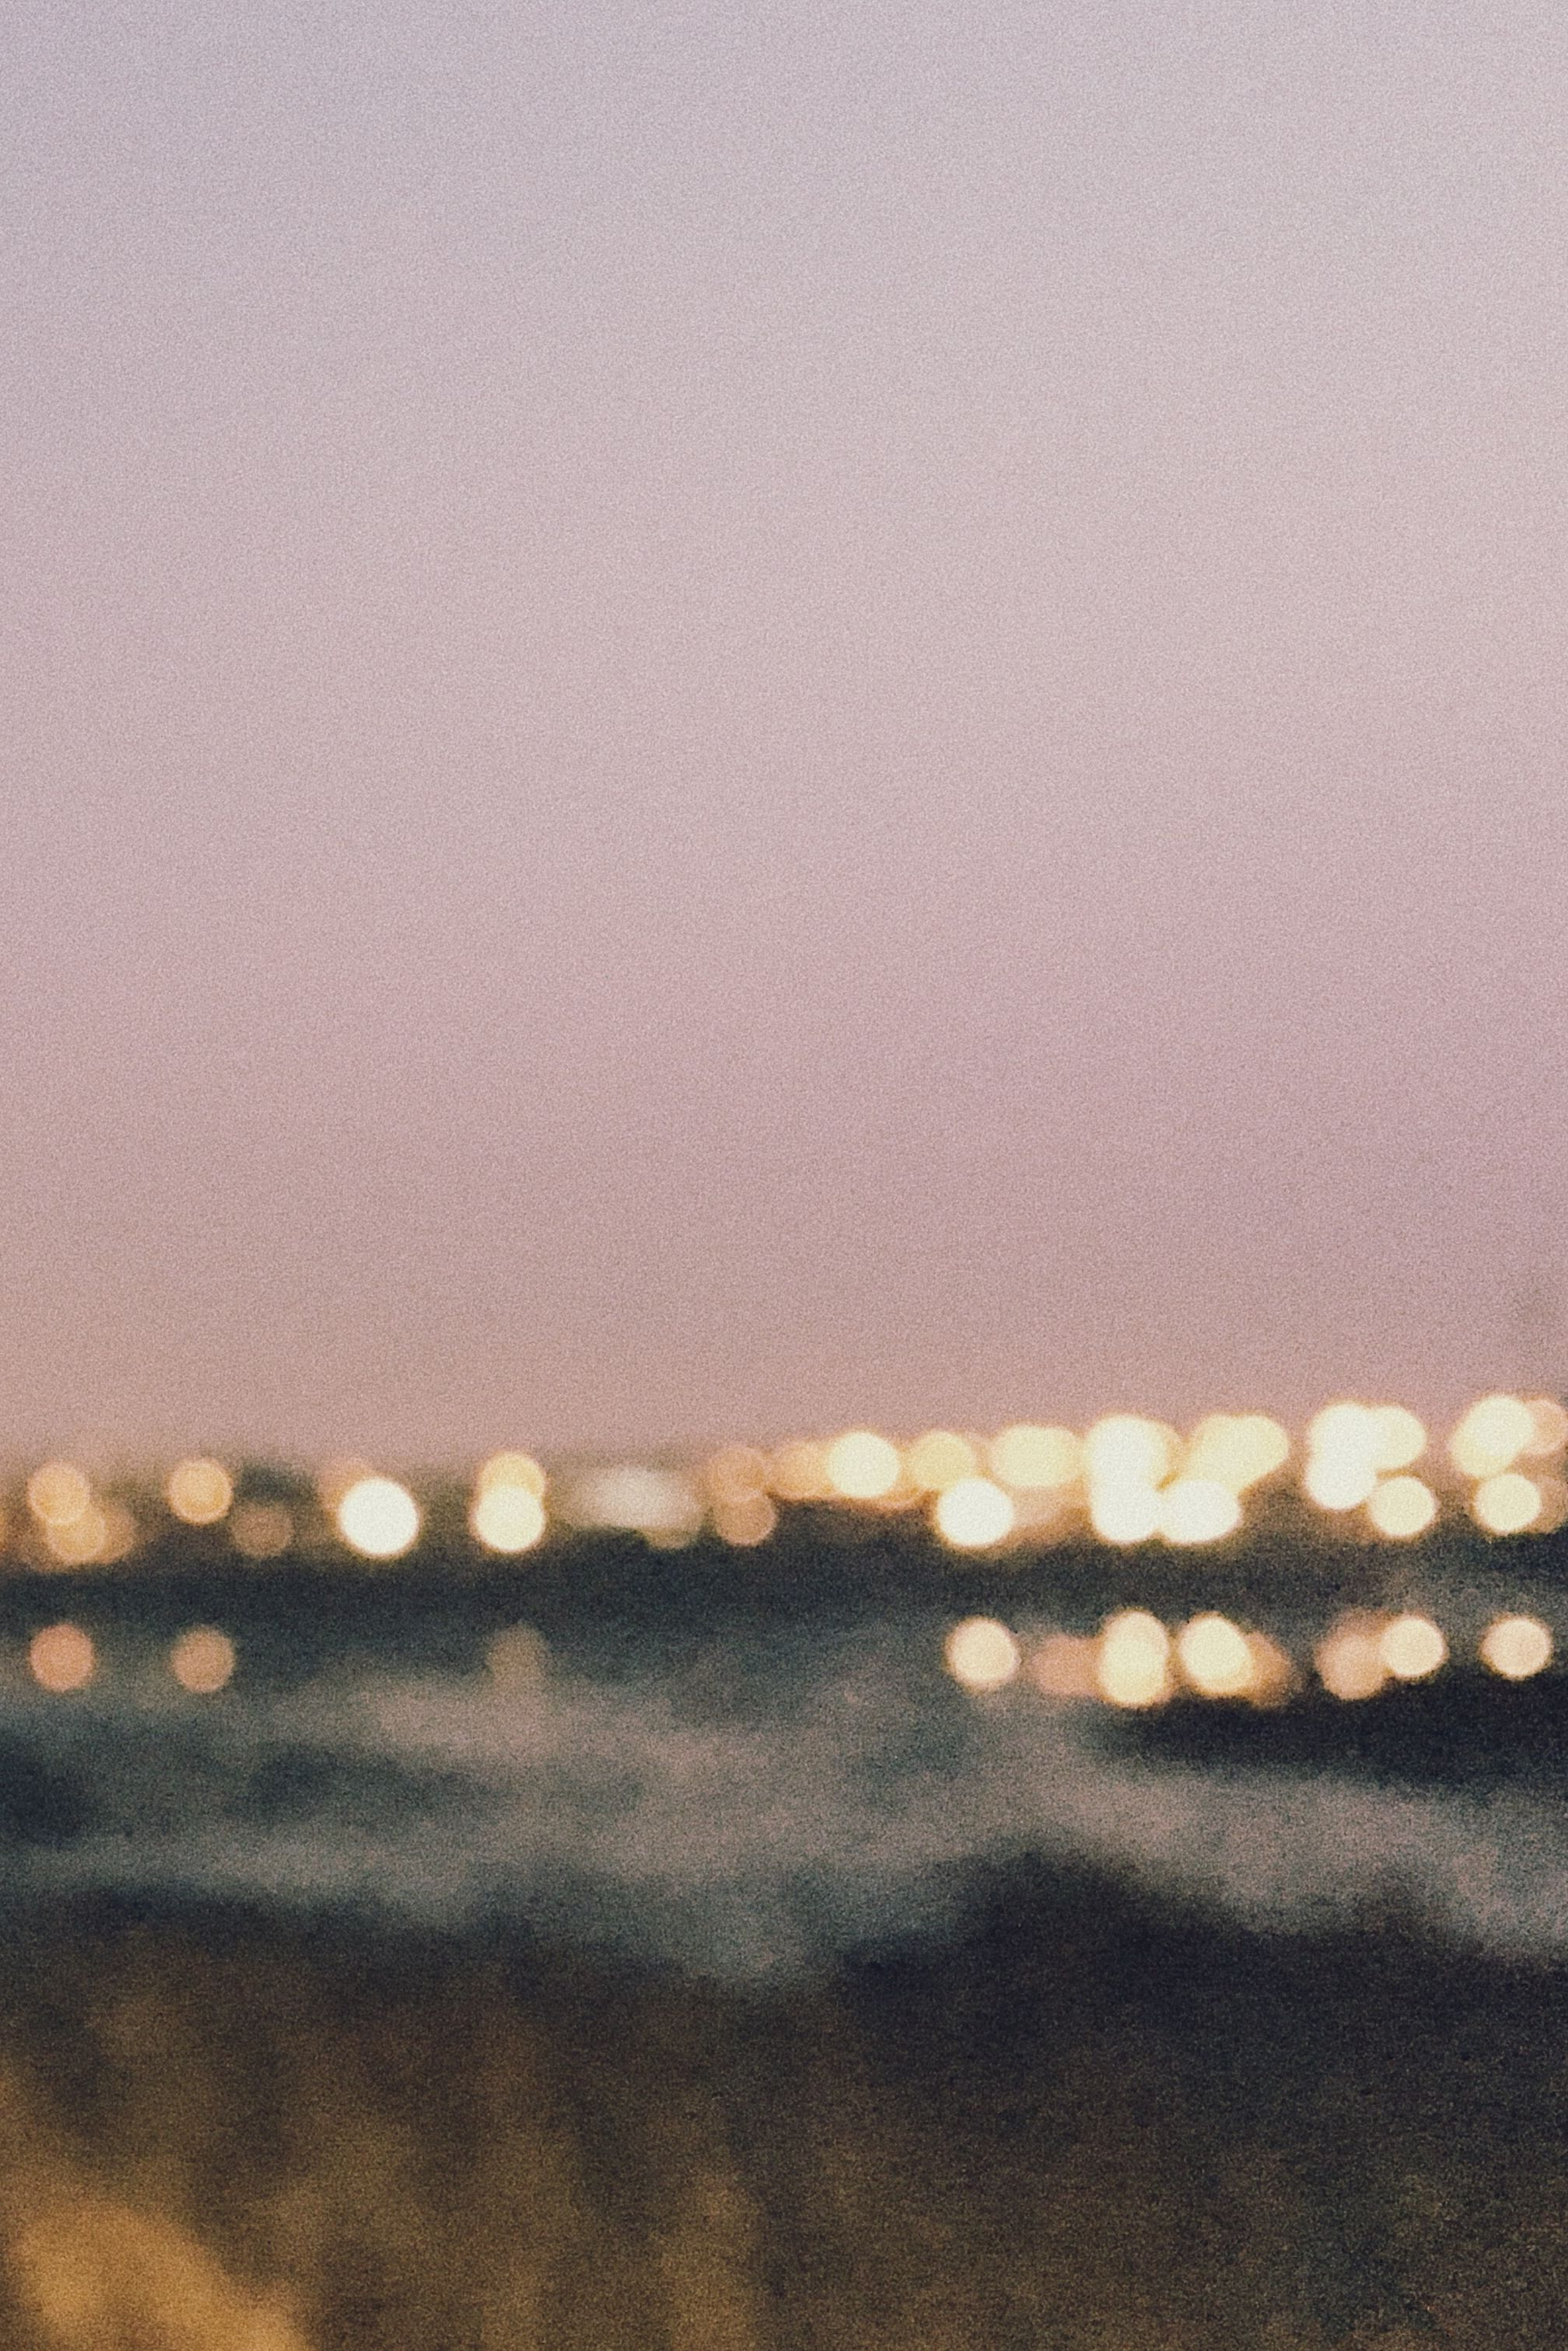
\includegraphics[width=\paperwidth, trim= 0cm 0cm 0cm 30cm]{blurry.jpg}}
\setbeamercolor{footnote}{fg=White}
\begin{frame}[plain]	
\titlepage
\end{frame}}

\begin{frame}{Which district is the most diverse?}

\begin{block}{\textbf{Diversity as variety (number of nationalities) per district}} Not very interesting... All districts have a similar amount of nationalities present (but possibly with only a few people!)
\end{block}

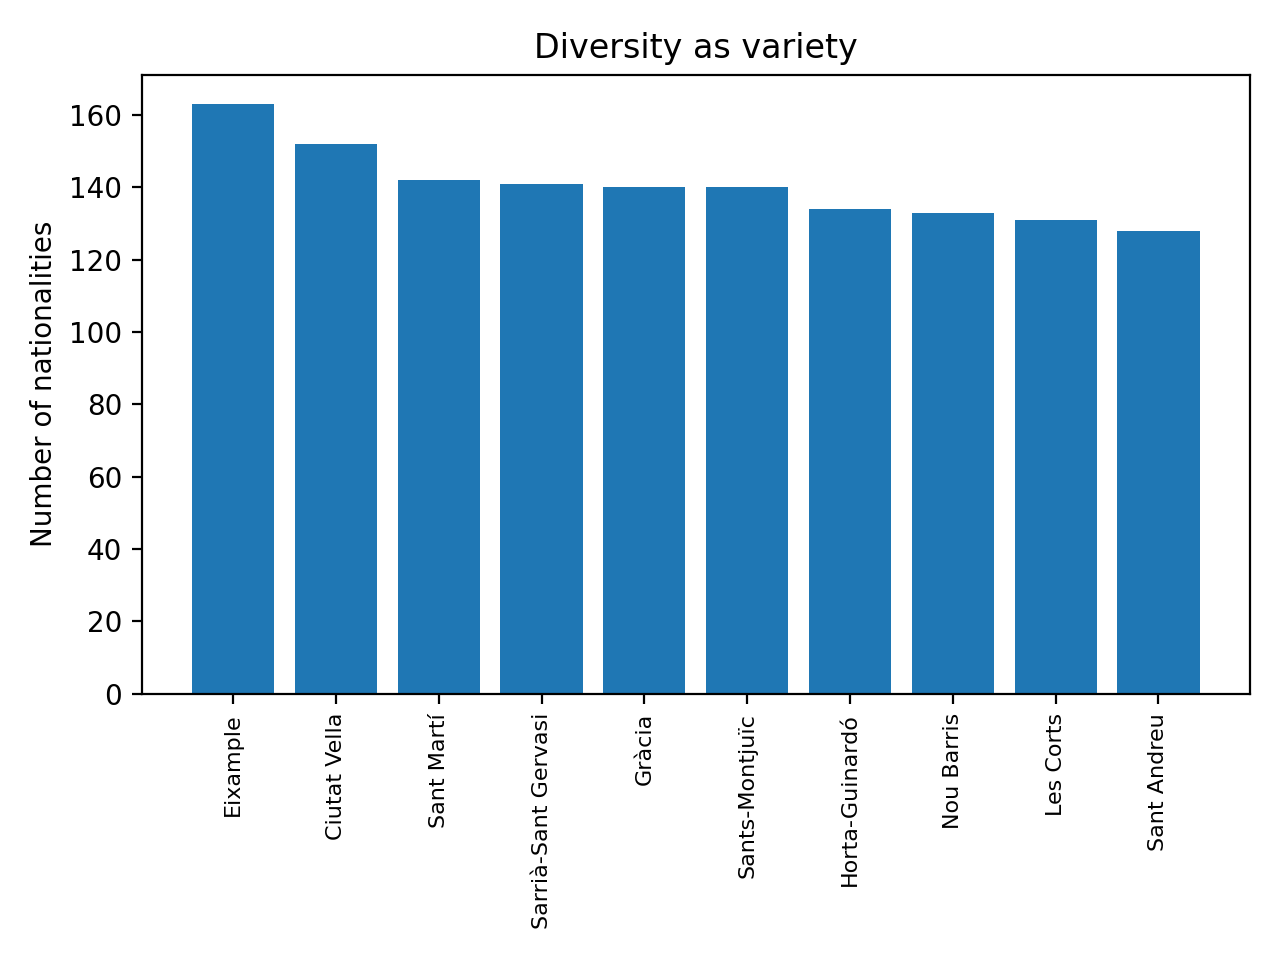
\includegraphics[width=9cm]{diversity_as_variety_districtes.png}



\end{frame}

\begin{frame}{Which district is the most diverse?}
\begin{block}{\textbf{Diversity as variety+balance per district}} 
Much more interesting! The Simpson index\footnote[0]{Simpson index=$1-\sum_{i=1}^{k}\frac{n_{i}(n_{i}-1)}{N(N-1)}$} takes into account how many people of each nationality there are (as well as the amount of nationalities).
\end{block}

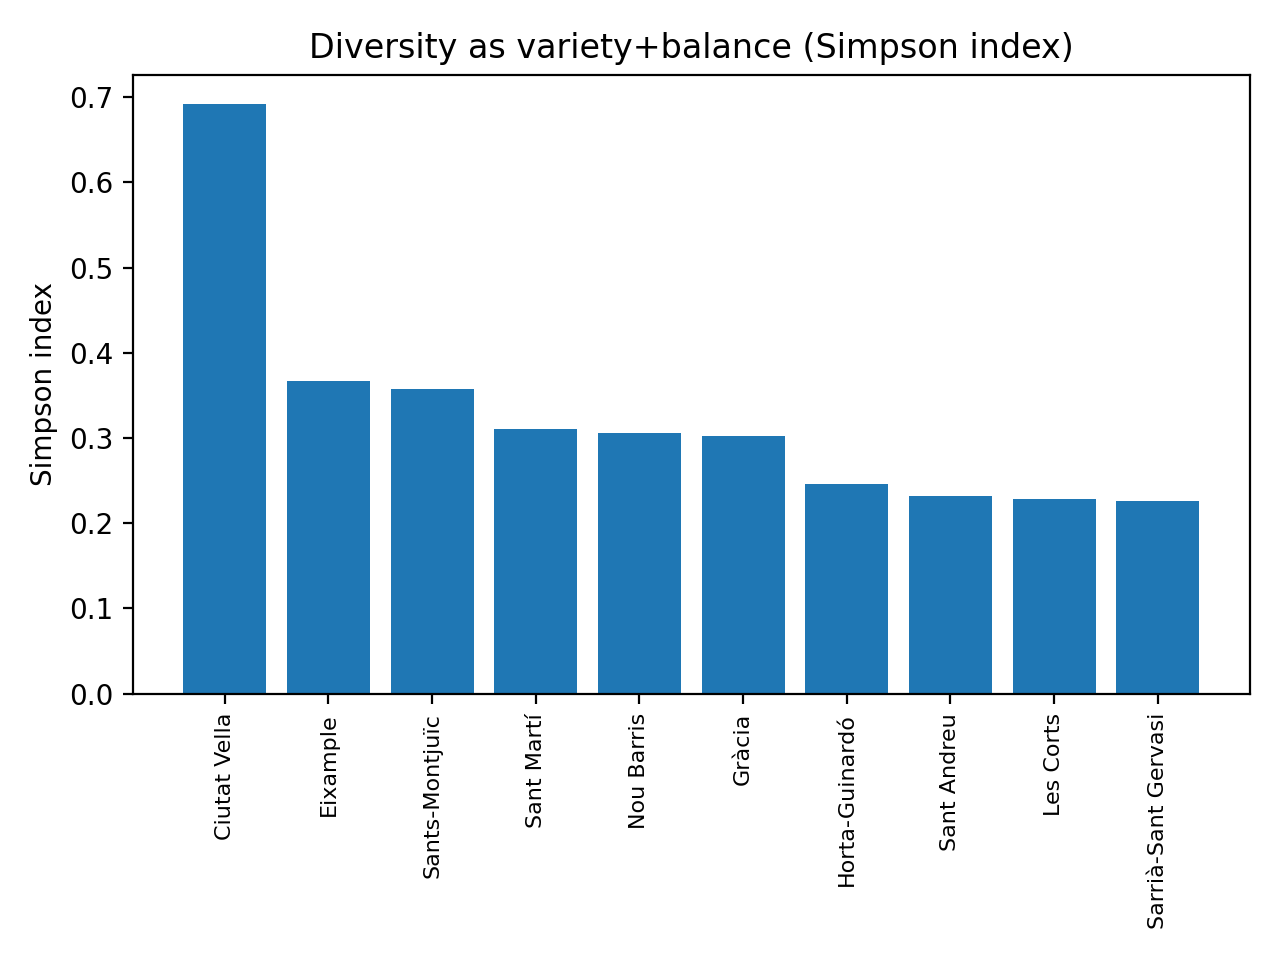
\includegraphics[width=9cm]{diversity_simpson_districts.png}

\end{frame}


\begin{frame}{Which district is the most diverse?}

\begin{block}{\textbf{Percentage of non-Spanish residents per district}} 
Also interesting. Conclusion: Ciutat Vella is by far the most diverse neighbourhood and also the one with the most non-Spanish people.
\end{block}

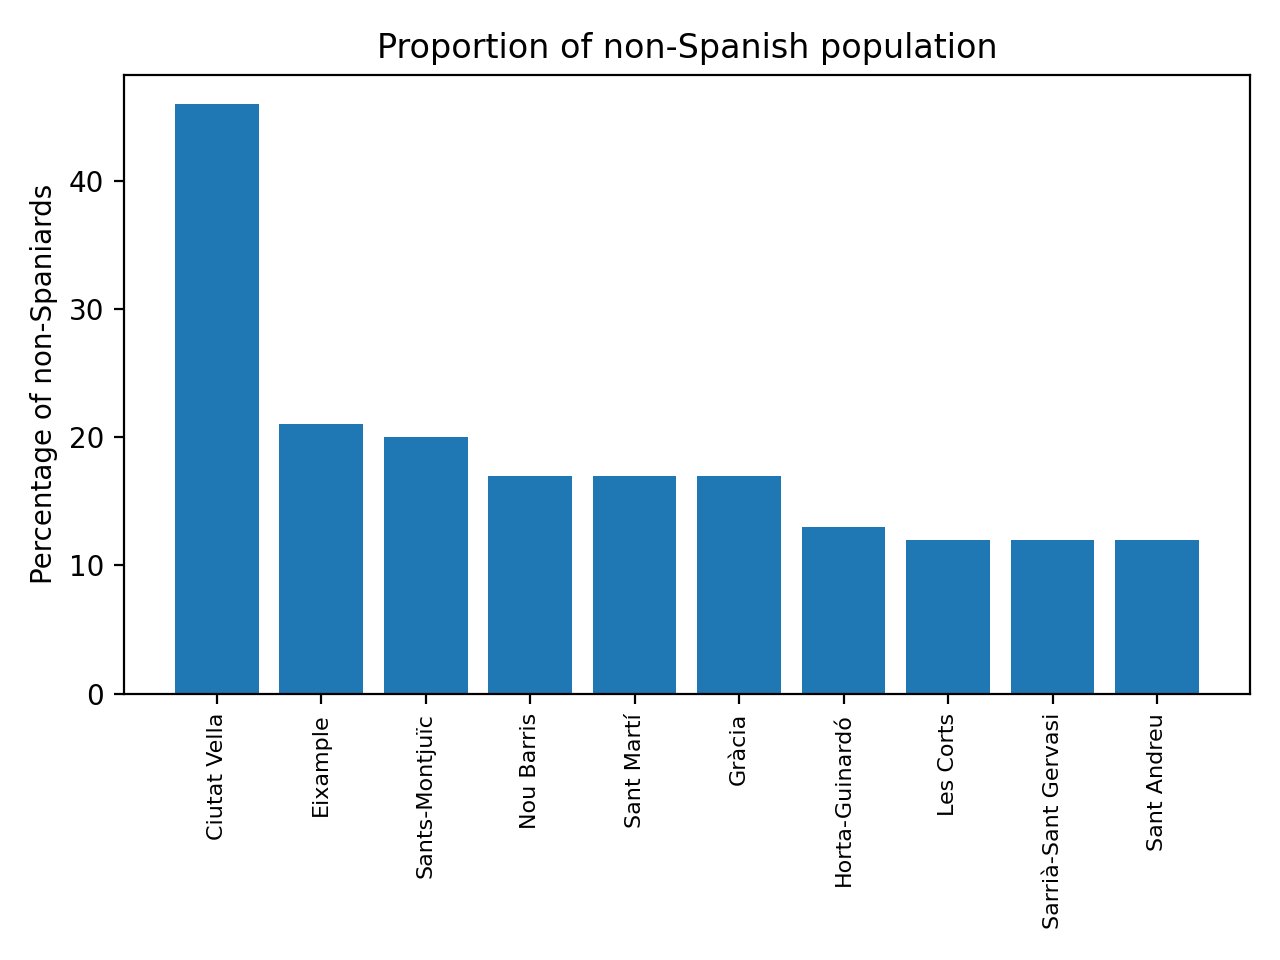
\includegraphics[width=9cm]{proportion_non_spanish_districts.png}

\end{frame}


\begin{frame}{Which neighborhood is the most diverse?}

\begin{block}{\textbf{Diversity as variety per neighborhood}}
Similarly to the case of districts: not super interesting.
\end{block}

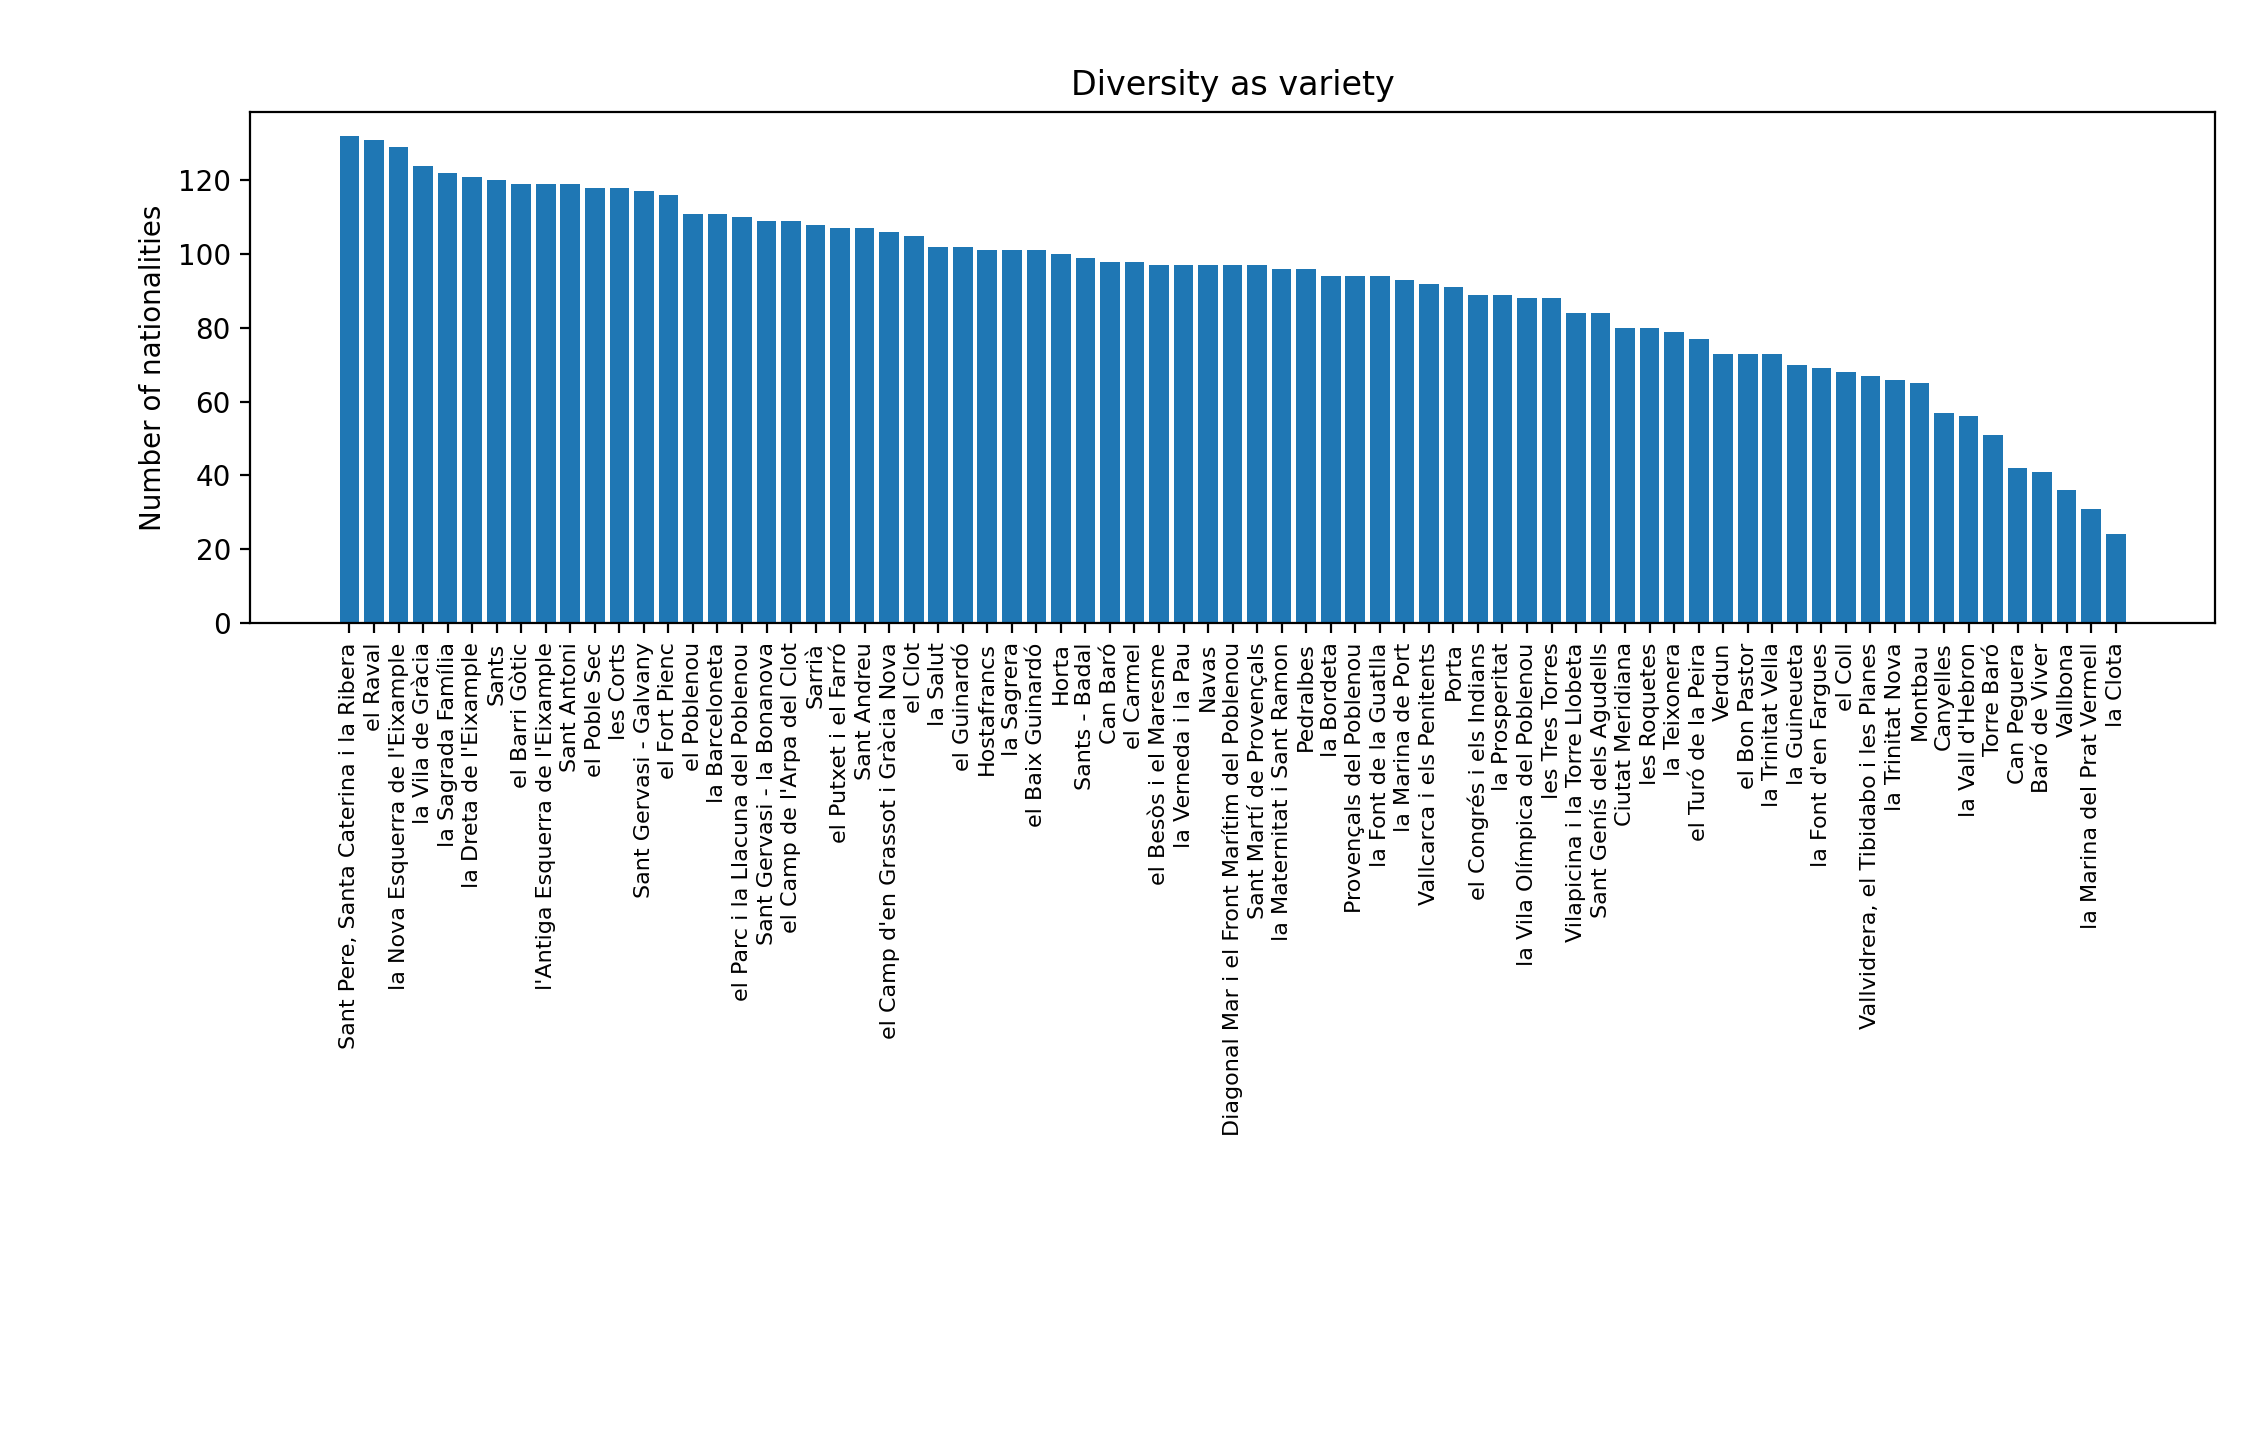
\includegraphics[width=12cm, trim= 3cm 4cm 0cm 0cm]{diversity_as_variety_barris.png}


\end{frame}


\begin{frame}{Which neighborhood is the most diverse?}

\begin{block}{\textbf{Diversity as variety+balance per neighborhood} }
As before, this is much more illuminating.
\end{block}

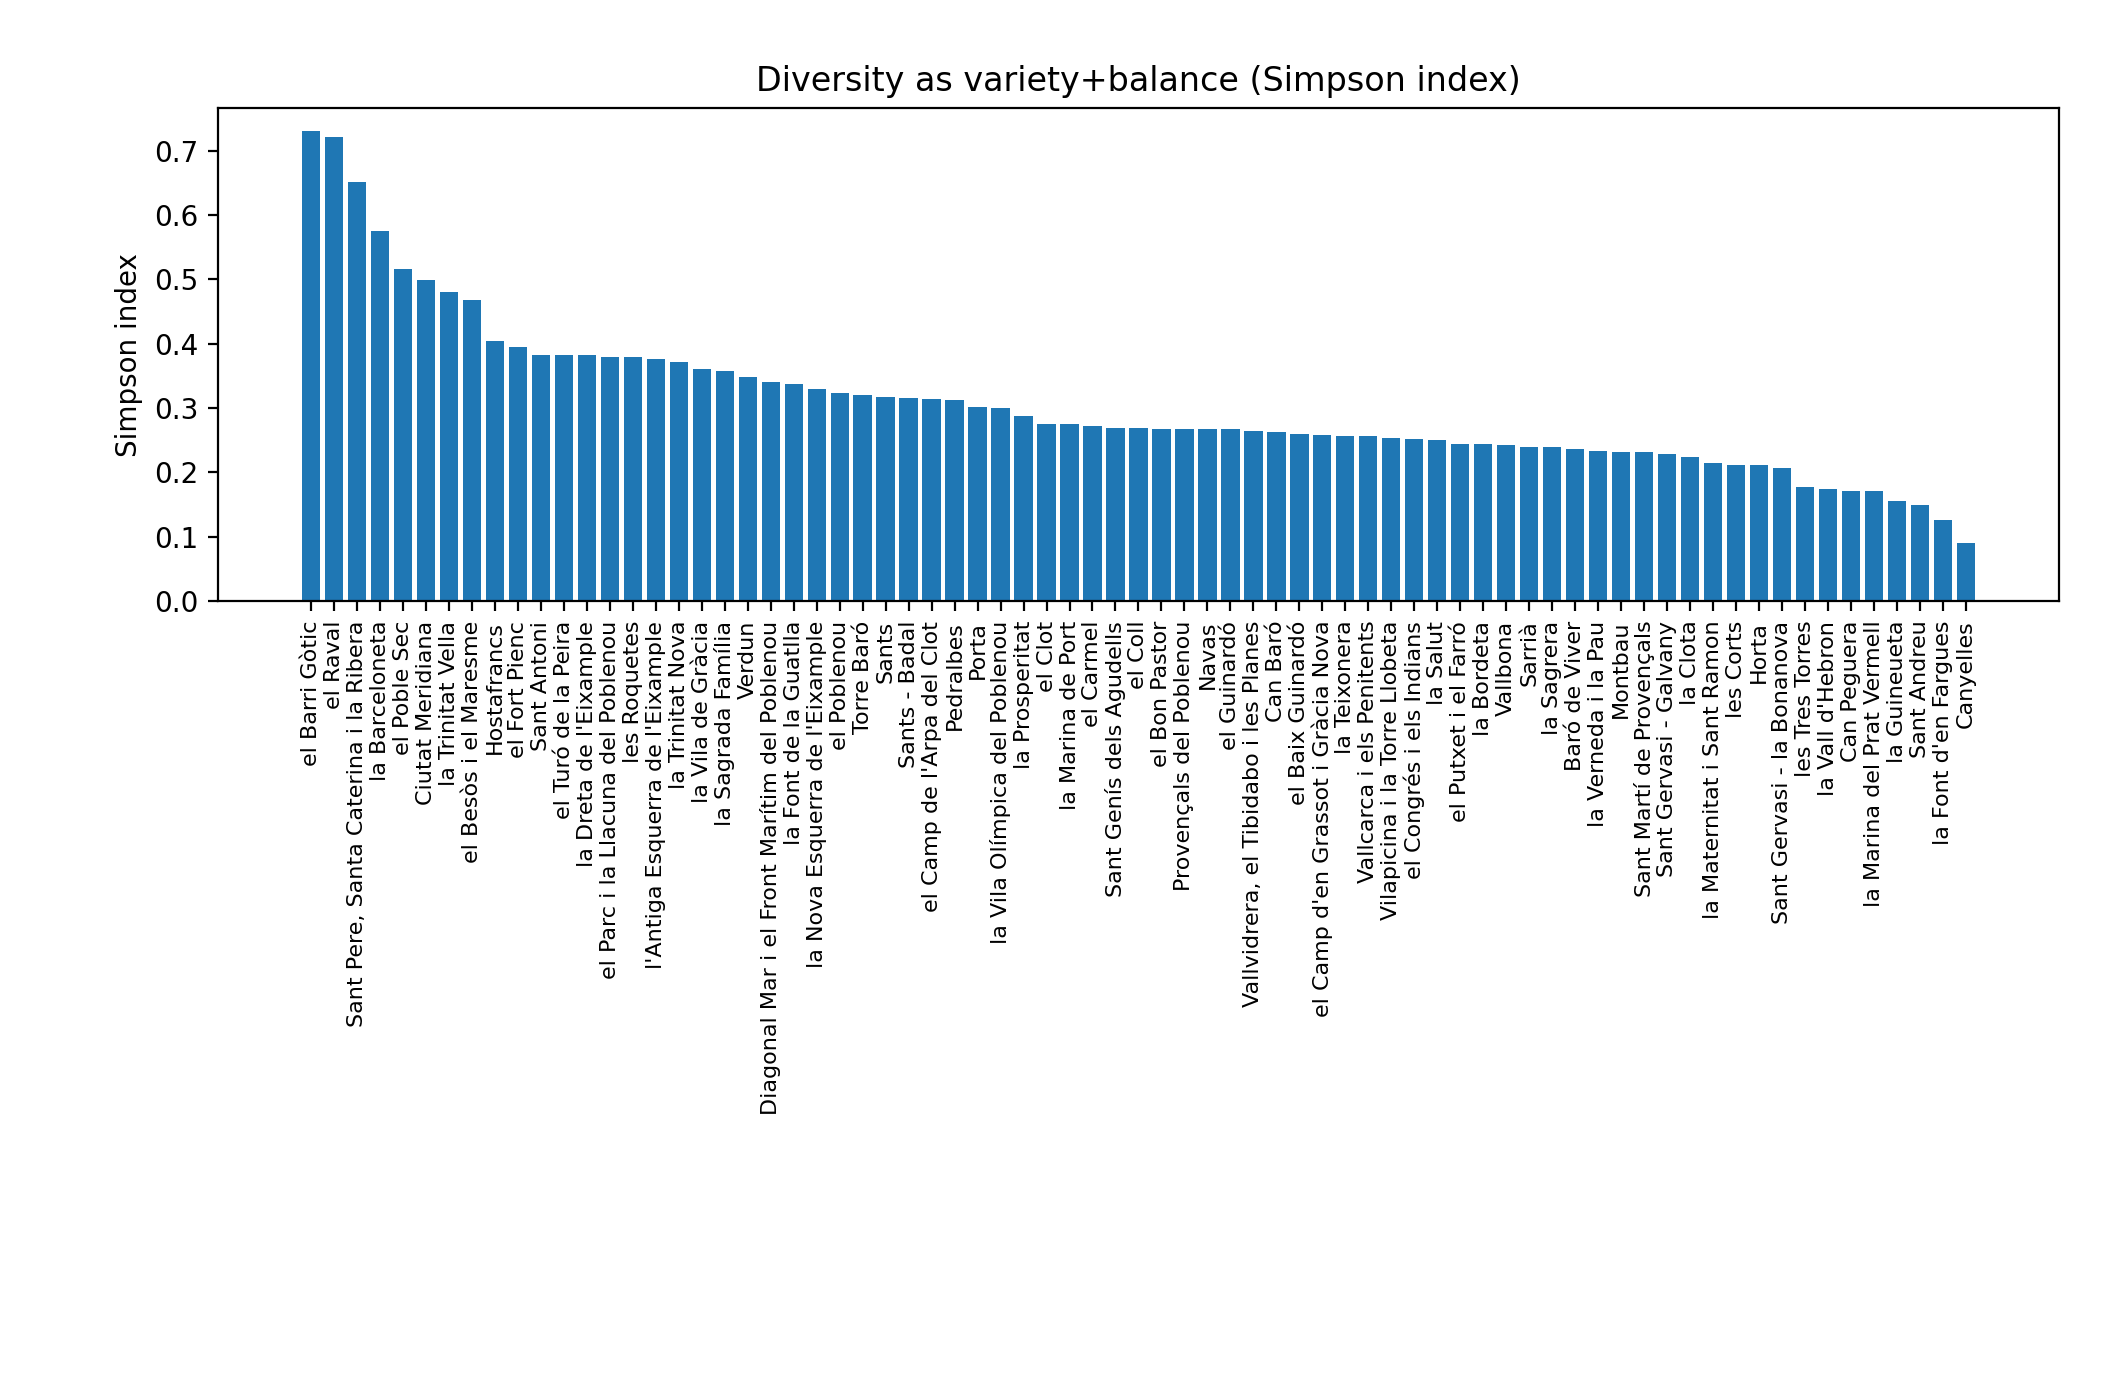
\includegraphics[width=12cm, trim= 3cm 4cm 0cm 0cm]{diversity_simpson_barris.png}

\end{frame}

\begin{frame}{Which neighborhood is the most diverse?}

\begin{block}{\textbf{\% of non-Spanish residents per neighborhood}} 
Interestingly, the neighborhoods that are the most diverse are those in the city center, followed by three suburban neighbourhoods: Ciutat Meridiana, Trinitat Vella and Bes\`{o}s i el Maresme.
\end{block}

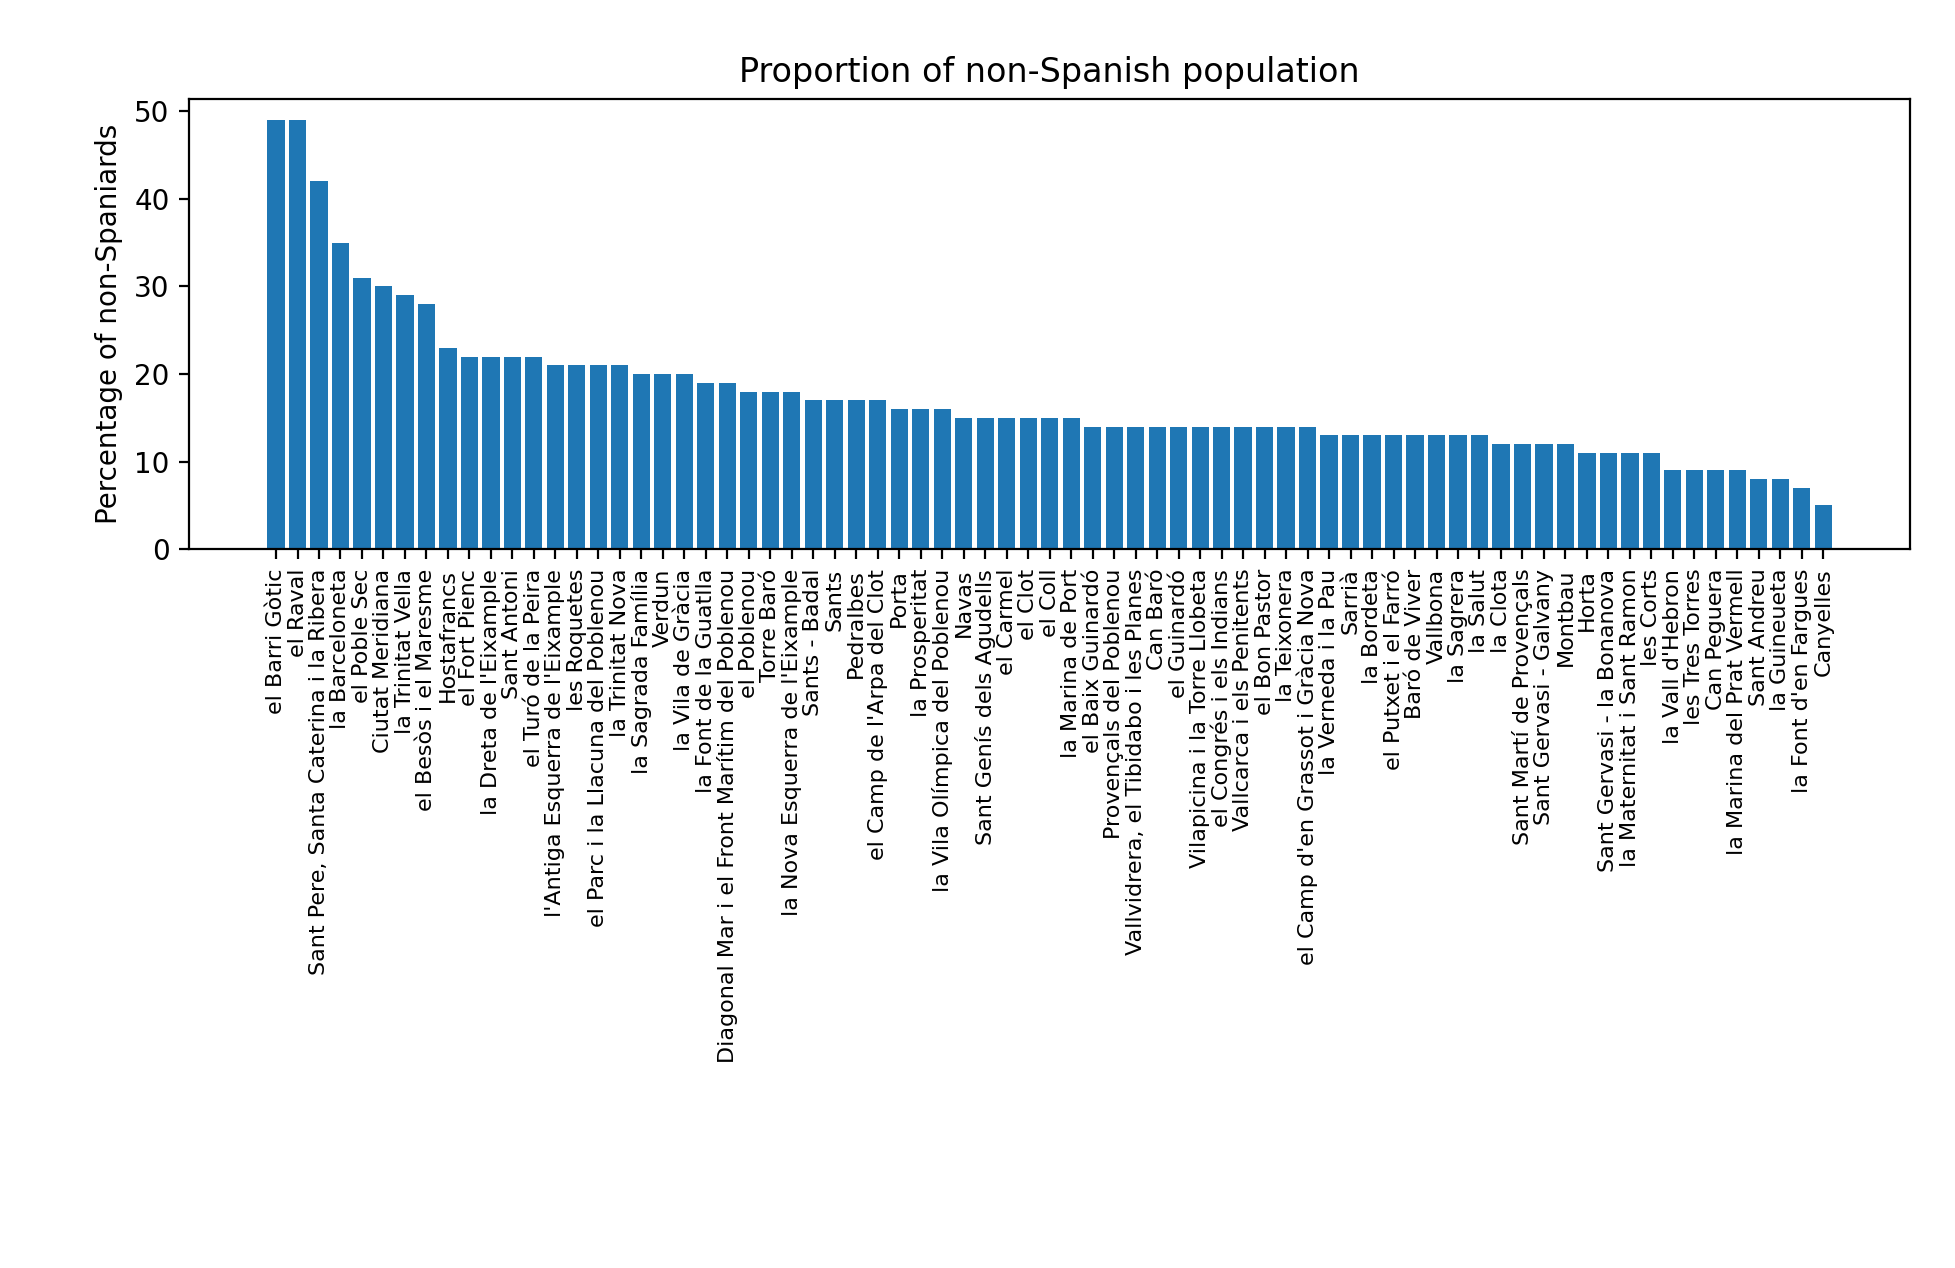
\includegraphics[width=12cm, trim= 2.8cm 4cm 0cm 0cm]{proportion_non_spanish_neighborhoods.png}


\end{frame}

\begin{frame}{Are there nationalities with a higher concentration of women?}

\begin{block}{\textbf{\% of women per nationality (for nationalities with more than 5000 people)}} 
There are huge differences among different nationalities. Many central and south American nationalities are amongst those with a higher \% of women.
\end{block}

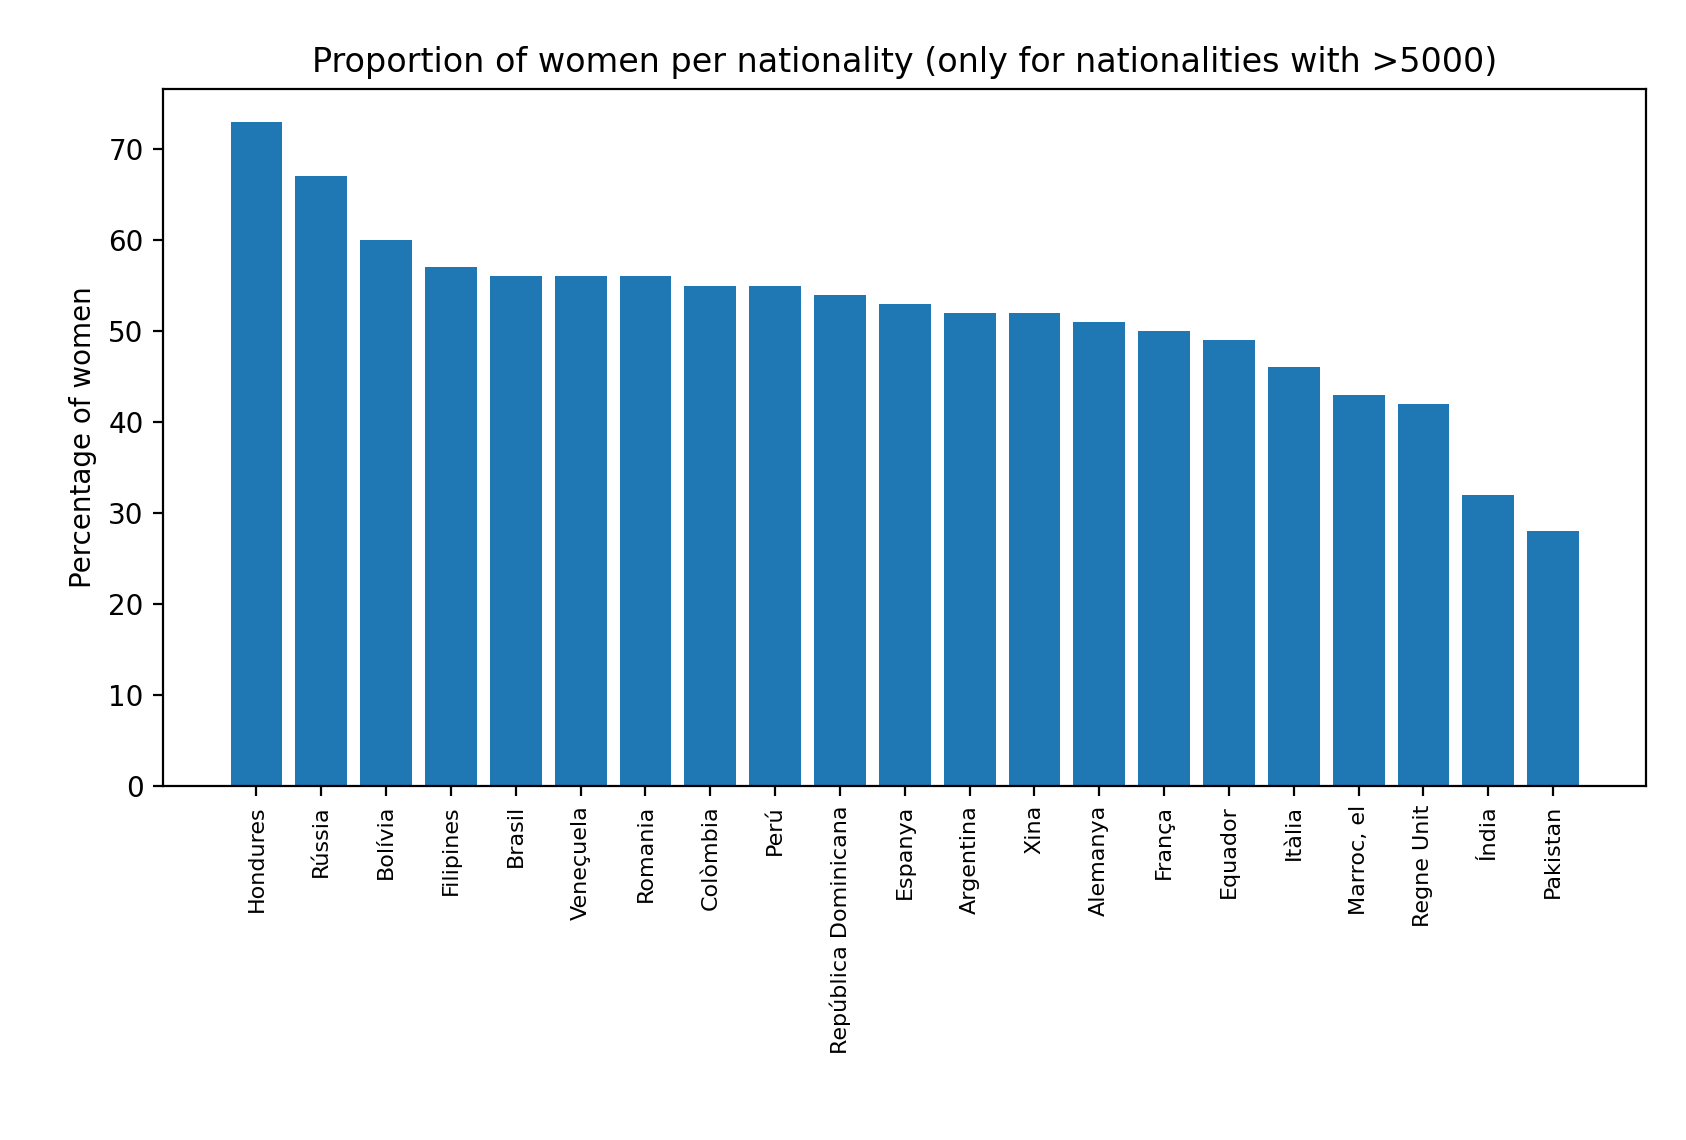
\includegraphics[width=11cm, trim= 2cm 0cm 0cm 0cm]{proportion_gender_per_nationality.png}


\end{frame}

\begin{frame}{Are there districts with a higher percentage of women?}

\begin{block}{\textbf{\% of women per district}} 
Not very interesting... Women are quite evenly spread across the city.
\end{block}

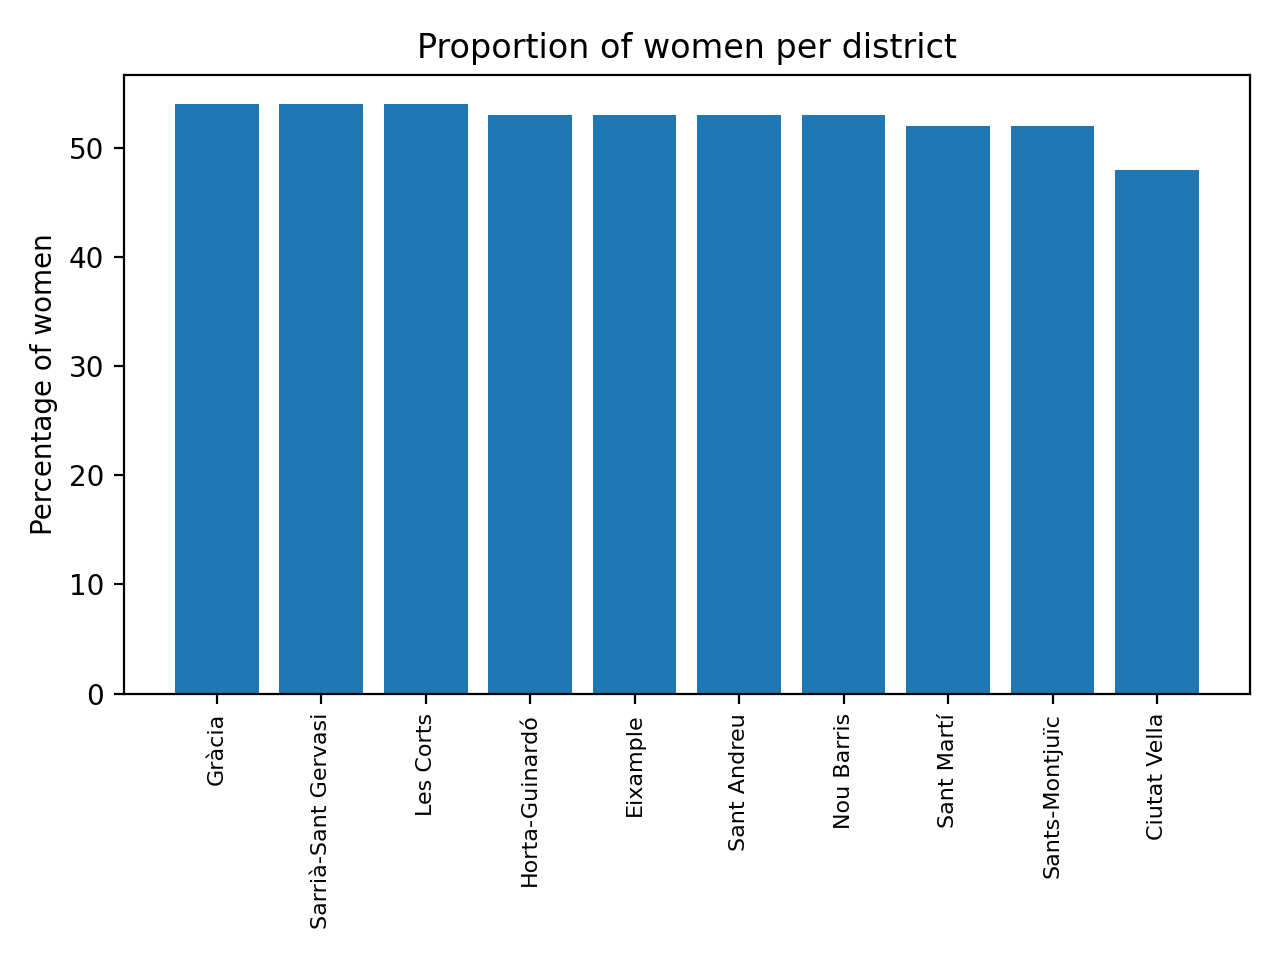
\includegraphics[width=10cm, trim= 0.5cm 0cm 0cm 0cm]{proportion_women_districts.png}
\end{frame}



\begin{frame}{Are there neighborhoods with a higher percentage of women?}
\begin{block}{\textbf{\% of women per neighborhood}} 
Same.
\end{block}

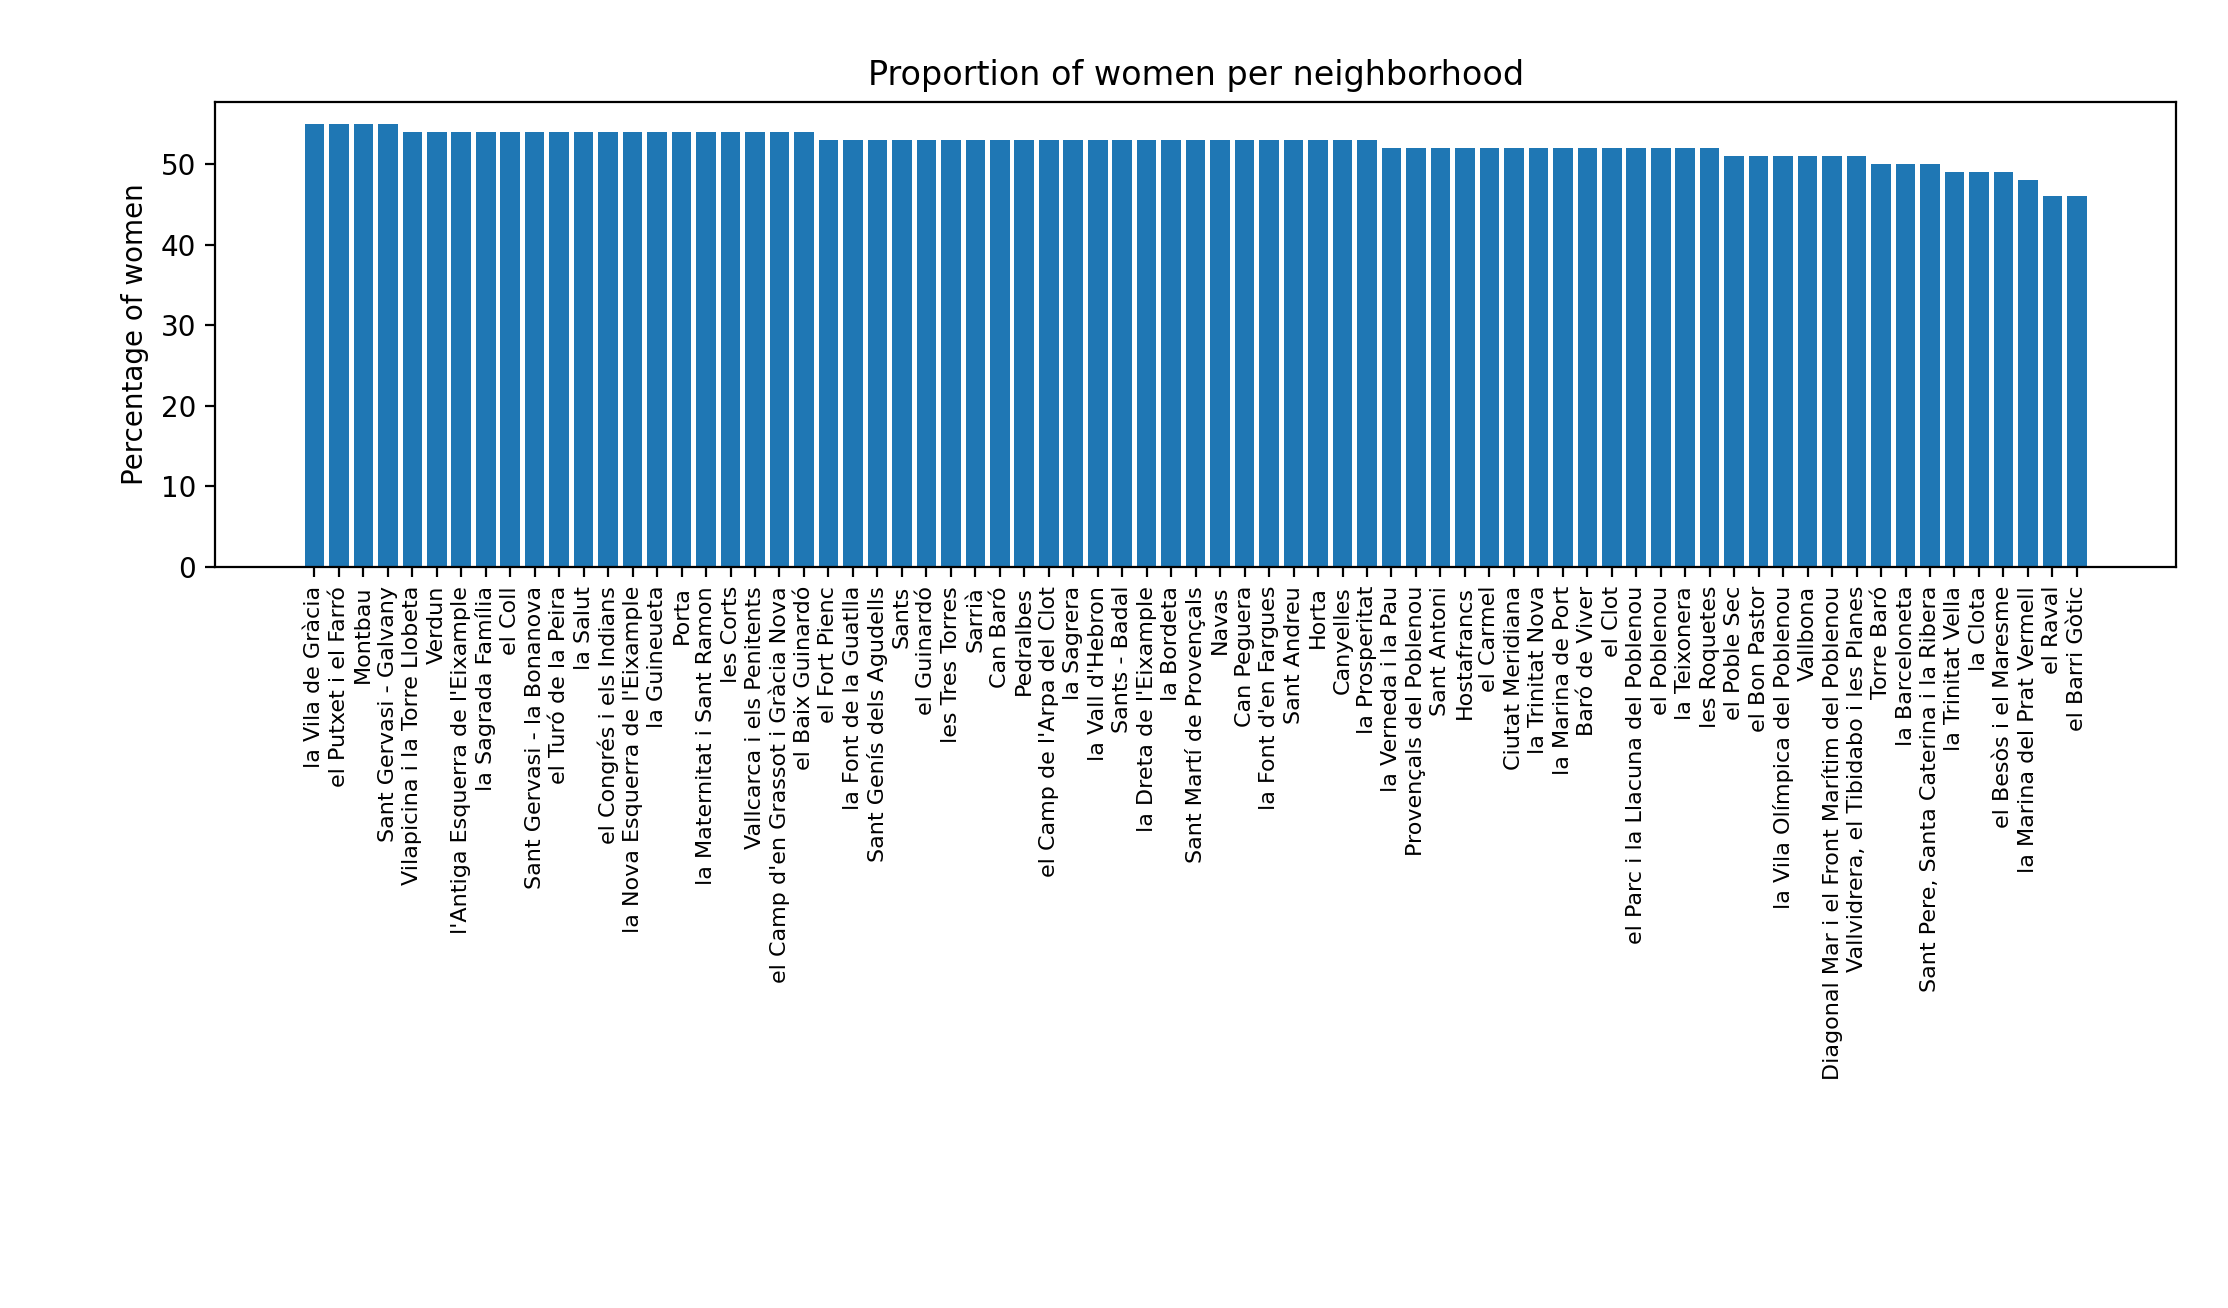
\includegraphics[width=12cm, trim= 3cm 0cm 0cm 0cm]{proportion_women_neighborhoods.png}
\end{frame}



\begin{frame}{Additional study 1: unemployment vs level of studies}
\begin{block}{\textbf{\% of unemployment vs percentage of people without any studies}} 
Interesting results. The common sense hypothesis that places with more people without studies are also those with higher unemployment levels is confirmed.
\end{block}

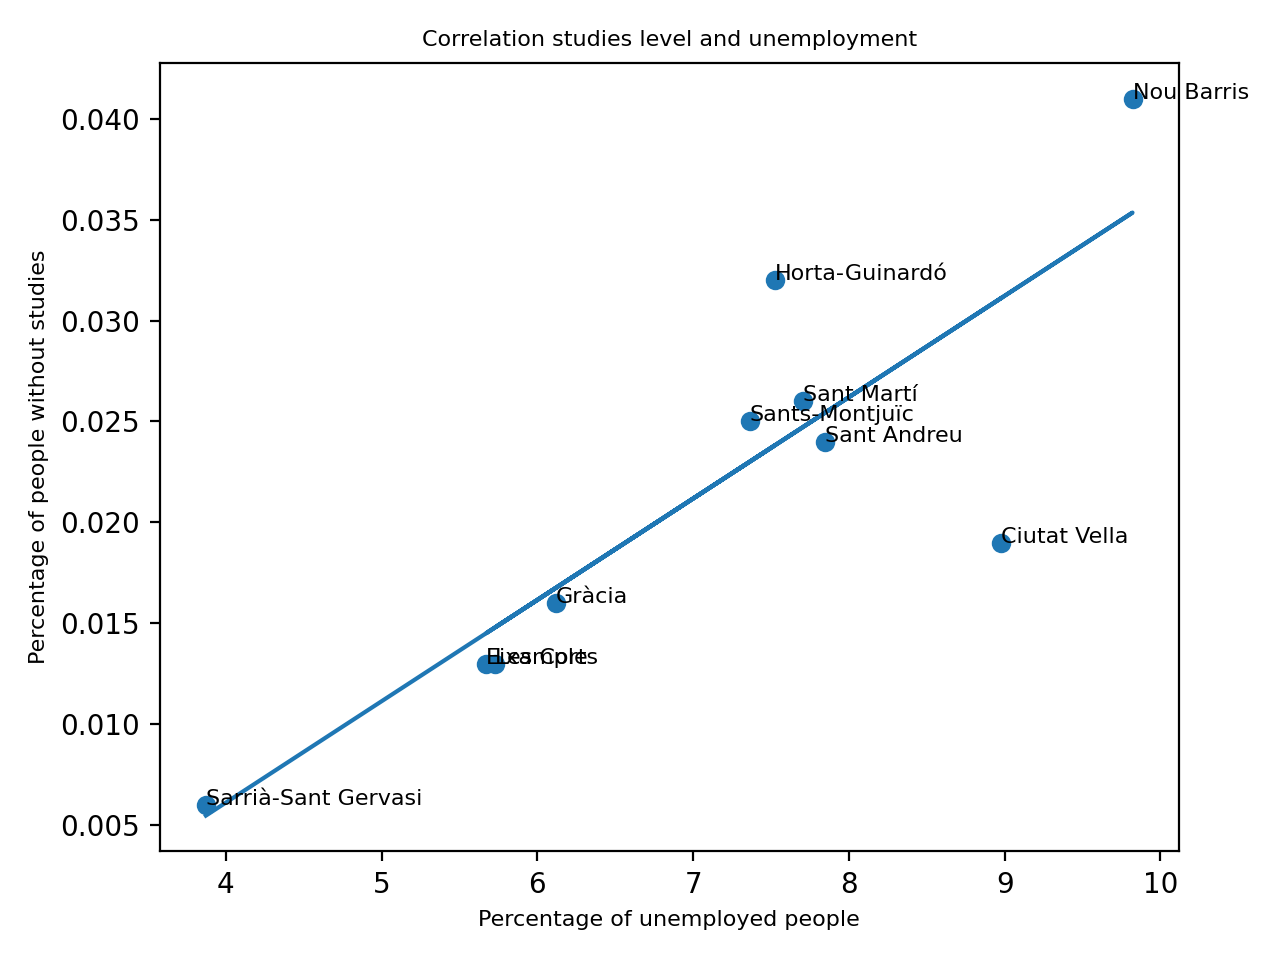
\includegraphics[width=10cm]{correlation_studies_level_unemployment_districts.png}

\end{frame}

\begin{frame}{Additional study 1: unemployment vs level of studies}

\begin{block}{\textbf{\% of unemployment vs percentage of people without any studies}} 
The trend is the same, but here we see that the neighbourhoods with the most people without studies do not have the highest unemployment. Hypothesis: these are `old' neighbourhoods where those people without studies are mostly retired.
\end{block}

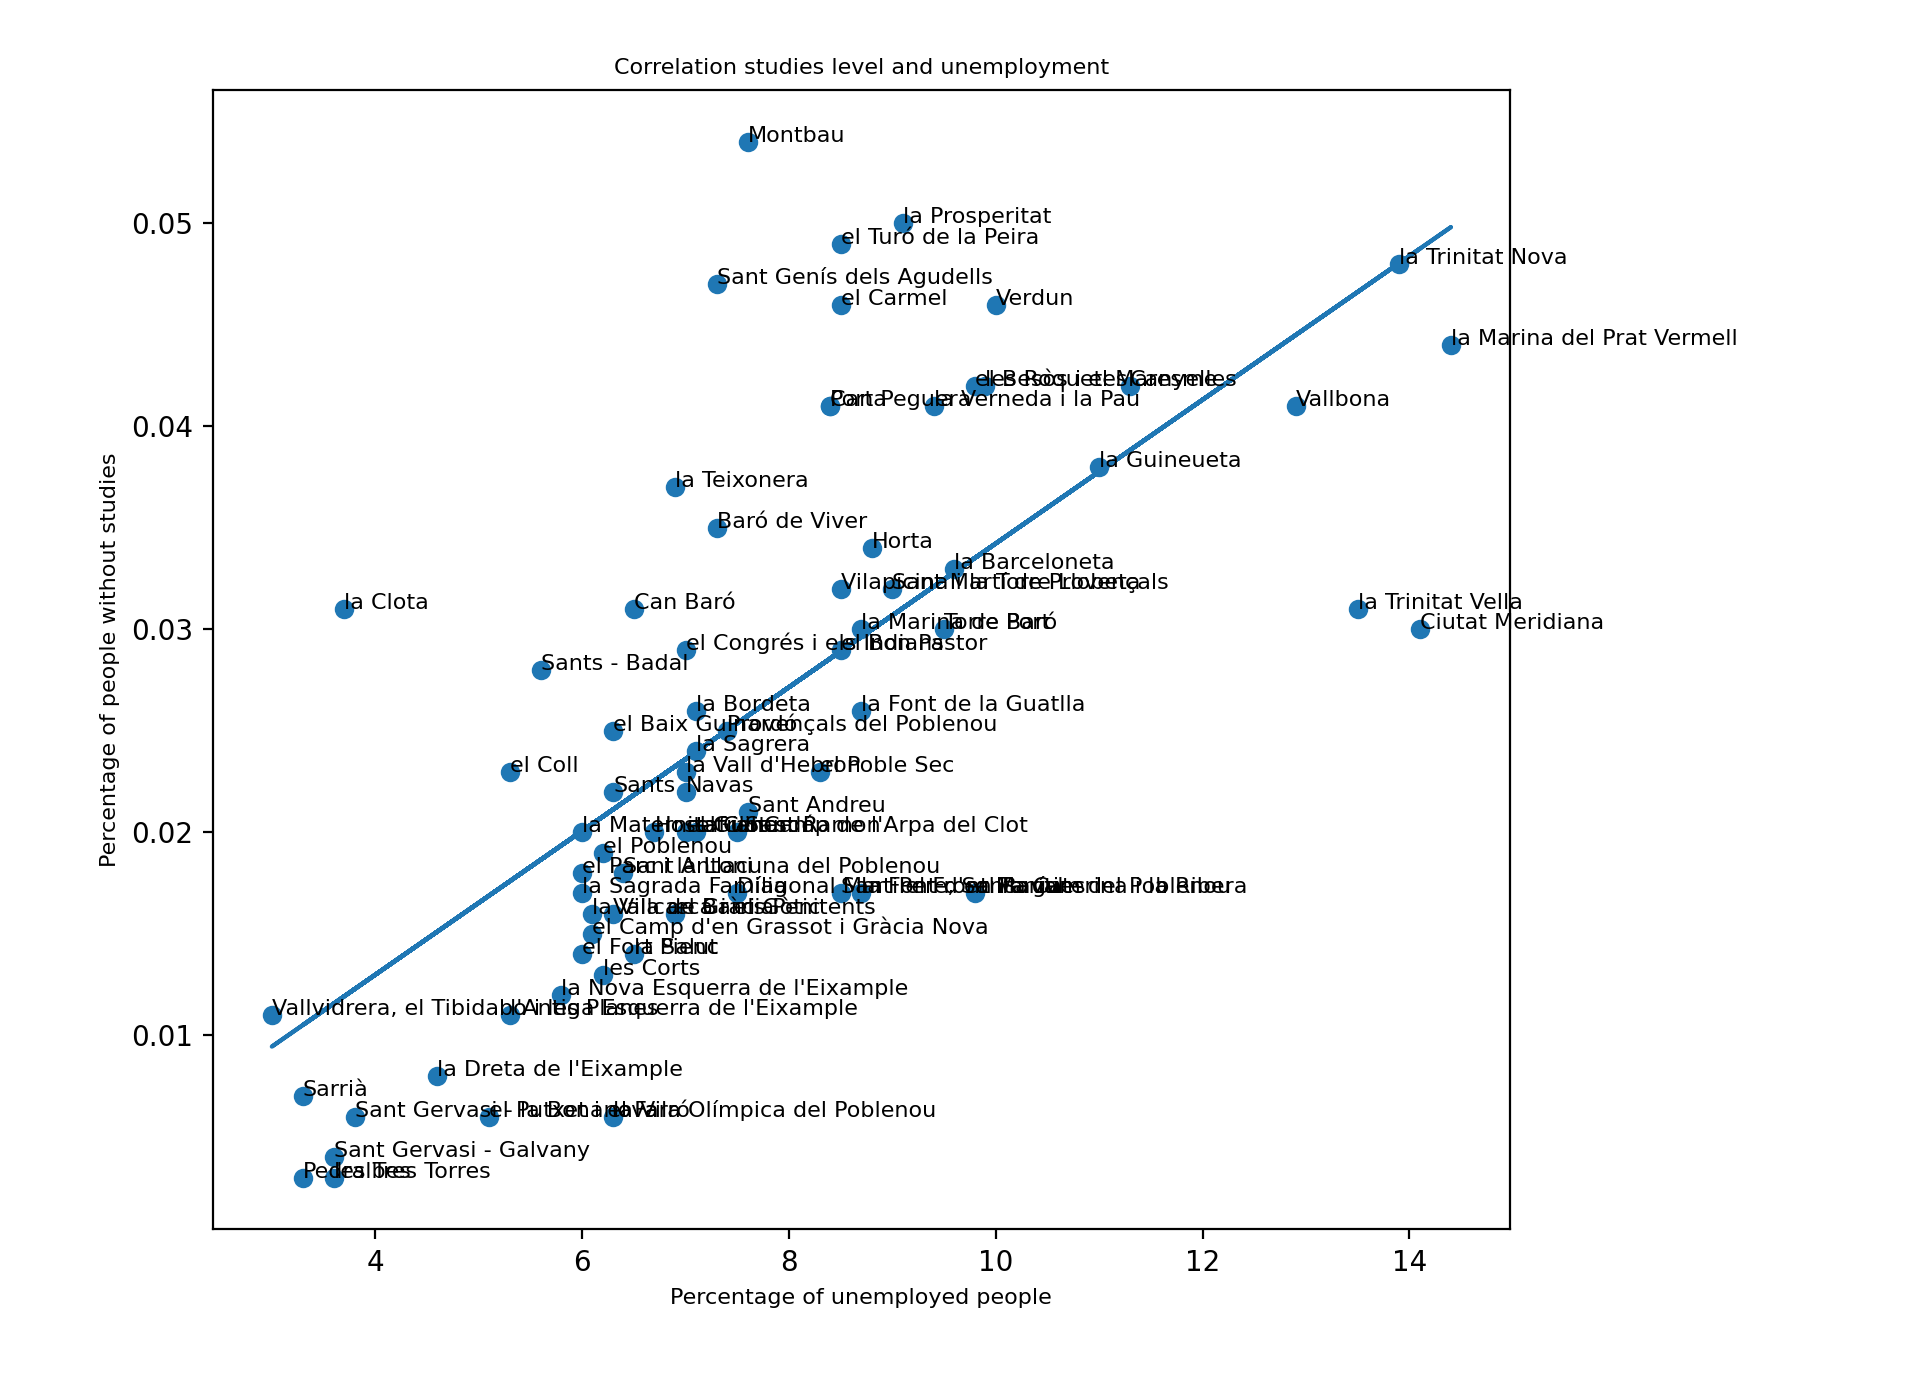
\includegraphics[width=10cm]{correlation_studies_level_unemployment_neighborhoods.png}



\end{frame}

\begin{frame}{Additional study 2: `bretxa tecnol\`{o}gica' vs usage of computers/wifi in public libraries}
\small{
\begin{block}{\textbf{\% of people without internet at home vs how much people use computers/wifi in public libraries}} 
Not very interesting. I thought there would be more of a correlation. Possible explanation: the data on the `bretxa tecnol\`{o}gica' is based on a survey and the survey could be incomplete.
\end{block}}

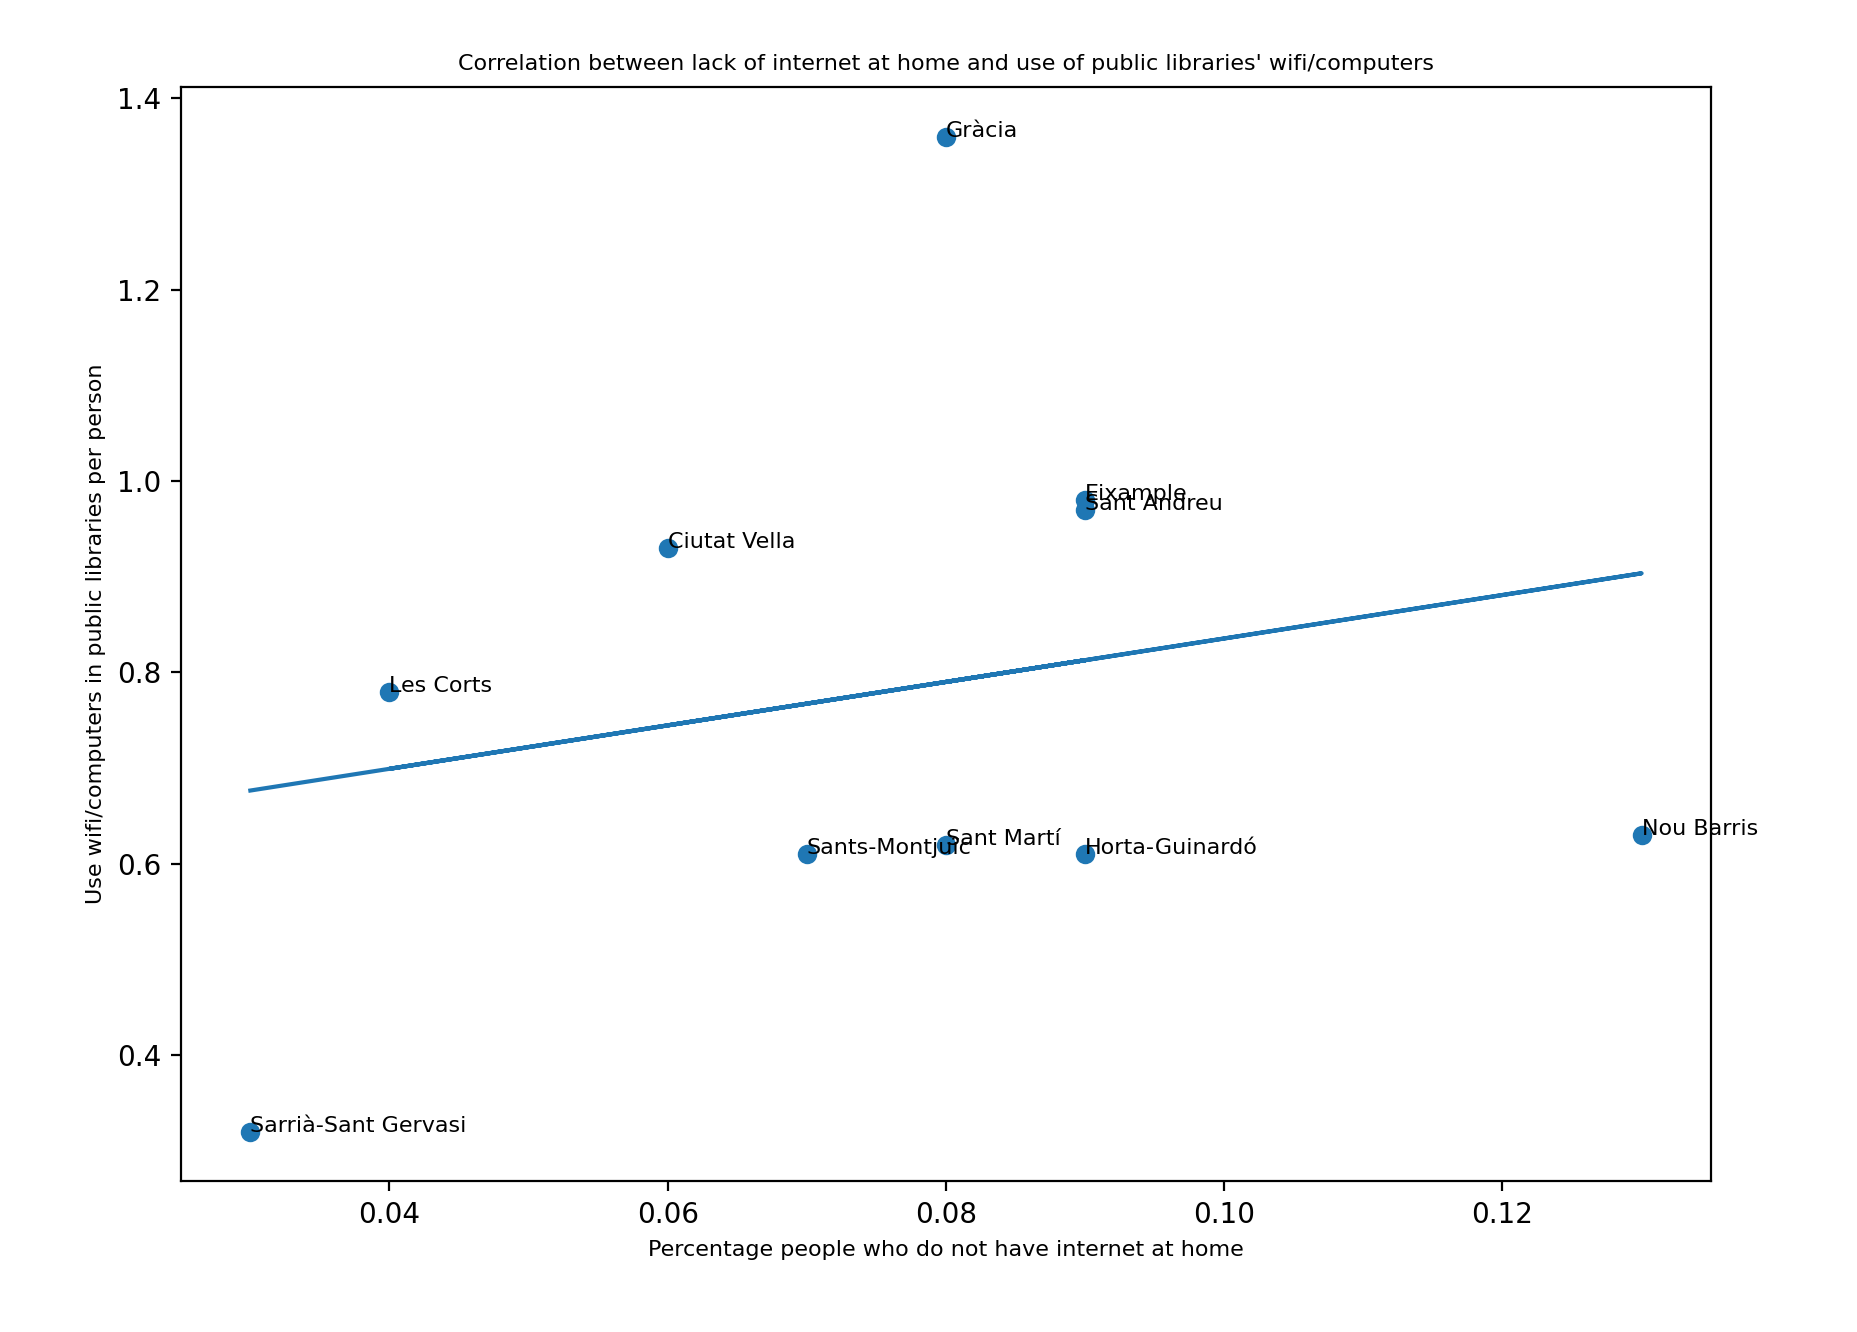
\includegraphics[width=9cm]{bretxa_tecno_biblioteques.png}



\end{frame}


\begin{frame}{Sources the for last two studies}

CSV files from Open Data BCN:

\begin{itemize}
\item `Pes del atur registrat de la població de 16 a 64 anys de la ciutat de Barcelona'

\item `Padró d'habitants. Població de la ciutat de Barcelona segons sexe i nivell acadèmic'

\item `Dades de la xarxa de biblioteques de la ciutat de Barcelona'

\item `Enquesta sobre la bretxa digital a la ciutat de Barcelona' (it was made in 2020, so it does not match the rest of data, which is all from 2018 -- but I assumed it was still significant)
\end{itemize}
\end{frame}




\end{document}
